Con la patinadora comenzando desde lo alto de la pista.  Marca en la pista debajo de cada grafica donde crees que se encuentra la patinadora para poder tener la energía que muestran los gráficos. Después comprueba con la simulación si tu predicción fue correcta.

\begin{table}[H]
    \centering
    \begin{tabular}{|p{1.8cm}|c|c|c|c|}
        \hline
                                            & 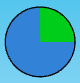
\includegraphics[width=50pt]{../images/pie}    & 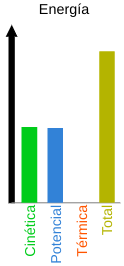
\includegraphics[width=50pt]{../images/bars}   & 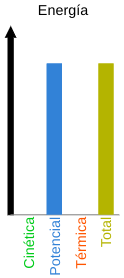
\includegraphics[width=50pt]{../images/bars_potential} & 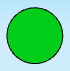
\includegraphics[width=50pt]{../images/pie_green} \\ \hline
        Dibuja la posición de la patinadora & 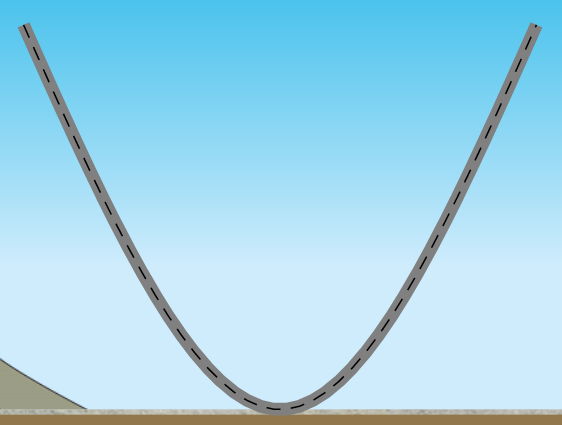
\includegraphics[width=100pt]{../images/pista} & 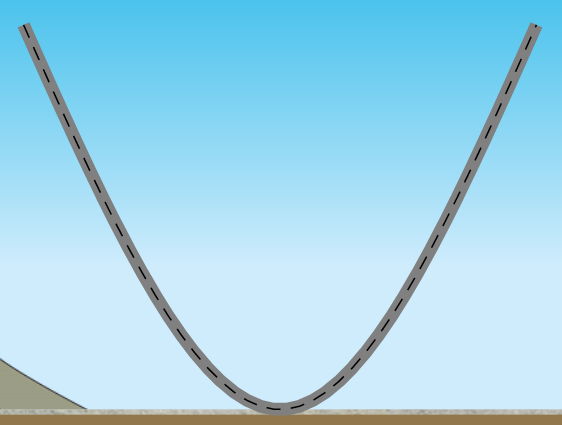
\includegraphics[width=100pt]{../images/pista} & 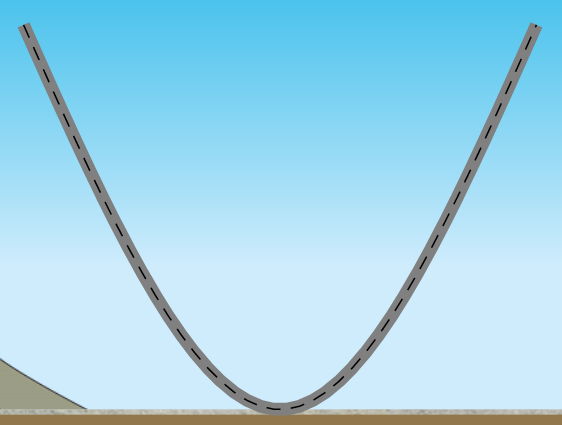
\includegraphics[width=100pt]{../images/pista}         & 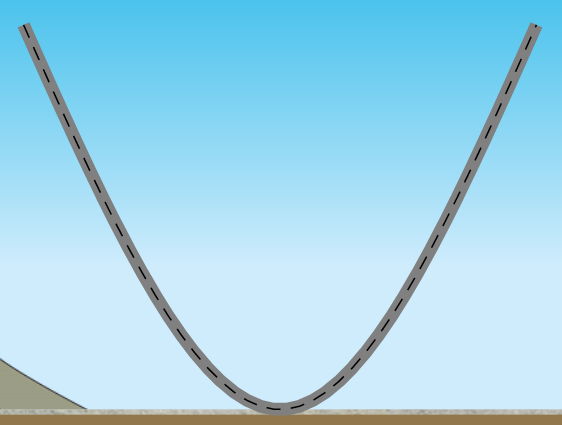
\includegraphics[width=100pt]{../images/pista}    \\ \hline
    \end{tabular}
    \label{tab:q25}
\end{table}